%%
%% 研究報告用スイッチ
%% [techrep]
%%
%% 欧文表記無しのスイッチ(etitle,eabstractは任意)
%% [noauthor]
%%

%\documentclass[submit,techrep]{ipsj}
\documentclass[submit,techrep,noauthor,dvipdfmx]{ipsj}

\usepackage{graphicx}
\usepackage{latexsym, url,dtk-logos}
\usepackage{color}
\usepackage{newtxtext, newtxmath}
\usepackage{bmpsize}
\usepackage{multirow}

\def\Underline{\setbox0\hbox\bgroup\let\\\endUnderline}
\def\endUnderline{\vphantom{y}\egroup\smash{\underline{\box0}}\\}
\def\|{\verb|}
% 
% 参考文献スタイルの不整合による \newblock エラーの回避
\providecommand{\newblock}{\hskip .11em plus .33em minus .07em}
%

%\setcounter{巻数}{79}
%\setcounter{号数}{10}
%\setcounter{page}{100}

\usepackage[utf8]{inputenc} 	%波ダッシュ（〜）を表記できるようにする

% \def\Underline{\setbox0\hbox\bgroup\let\\\endUnderline}
% \def\endUnderline{\vphantom{y}\egroup\smash{\underline{\box0}}\\}
% \def\|{\verb|}
\usepackage{fancyvrb}
\renewcommand{\|}{\Verb|}
\newcommand{\vbarSafe}{\texttt{|}}

% マル○記号を使いたい場合------ 
%	○×〜 などは機種依存文字のため本文で直接は使えない
%	本文では \maru と書くようにする
%	cf) https://livingdead0812.hatenablog.com/entry/20161005/1475654232
\newcommand{\maru}{\raise0.2ex\hbox{\textcircled{\scriptsize{ }}}}
\newcommand{\nami}{$\sim$}

% ------------------------------------------
% ---- figure 環境で横に画像を並べる ------------------
%	cf) https://atatat.hatenablog.com/entry/cloud_latex18_subcaption
\usepackage[hang,small,bf]{caption}
\usepackage[subrefformat=parens]{subcaption}
\captionsetup{compatibility=false}
% ------------------------------------------

% ---- 添削用 ----------------------
\usepackage{../muselab-correction} % 添削用のマクロを定義しているパッケージ
% \usepackage[final]{muselab_correction} % 添削終了時は final オプションをつける
%	このパッケージを使うと，添削用のコメントが出力される
% ------------------------------------------

% ---- この論文オリジナル ------------
% 何度も使う固有名詞や変数などを定義しておくと後で修正・変更が楽
\newcommand{\midiEvent}{\modified{`MIDI\_EVENT`}{\texttt{MIDI\_EVENT}}}
\newcommand{\MainModule}{\modified{`MainModule`}{\texttt{MainModule}}}
\newcommand{\RandomMelodyGenerator}{\modified{`RandomMelodyGenerator`}{\texttt{RandomMelodyGenerator}}}
\newcommand{\SheetOne}{\modified{`Sheet1`}{\texttt{Sheet1}}}
\newcommand{\WorksheetChange}{\modified{`Worksheet\_Change`}{\texttt{Worksheet\_Change}}}
\def\avoidnote{スケール外音符出現確率}
% ------------------------------------------


% ==============================================
% 引用文を整形する
% ==============================================
\usepackage{tcolorbox}
\tcbuselibrary{listingsutf8} % 日本語を含む文章を扱う場合に便利
\newtcolorbox{musequote}{%
  colback=gray!10,    % 背景色（薄い灰色）
  colframe=black,     % 枠線の色
  boxrule=0.3mm,      % 枠線の太さ
  arc=.5mm,            % 角の丸み
  left=5mm,           % 内側の左余白
  right=5mm,          % 内側の右余白
  top=2mm,            % 内側の上余白
  bottom=2mm,         % 内側の下余白
  fontupper=\footnotesize
}
\newcommand{\from}[1]{\\\rightline{\small{---\textit{#1}}}}

\makeatletter
% 不要な英文表記と受付日を消すための再定義
\renewcommand{\authortitle}{%
  {\jtitlefont\@title\par}%
  \vskip\Jtitlejauthorsep%
  {\authorfont\authoroutput{}\par}%
  % 受付日（\@uketsuke）の表示を削除
  \vskip\Jauthorjreceivesep%
  \vskip\Jreceivejabstsep%
  \mbox{\box\@abstractbox}\par%
  \vskip\Jabstsepjkeyword%
  \mbox{\box\@jkeywordbox}\par%
  \vskip\JEhonbunsep%
  % 以降の英文パート（タイトル、著者、受付日、アブストラクト）をすべて削除
}
\makeatother

\begin{document}


\title{% 卒業論文のタイトルを書く
持続音楽器におけるヴィブラート表現の整理と

教育的理解に向けた初期検討}

%\etitle{How to Prepare Your Paper for IPSJ SIG Technical Report \\ (version 2018/10/29)}
%SIGMUS/EC 予稿には入れるので，英文タイトルは考えておこう（情報学広場に掲載される英文タイトルがこれになる）

\affiliate{FU}{福知山公立大学情報学部}
% \affiliate{KW}{関西学院大学工学部}

\author{山崎 承太郎}{Yamasaki Jotaro}{FU}[32545100@fukuchiyama.ac.jp]
% \author{平山 心}{Hirayama Kokoro}{KW}[ifp34362@kwansei.ac.jp]
\author{橋田 光代}{Hashida Mitsuyo}{FU}[hashida-mitsuyo@fukuchiyama.ac.jp]

\begin{abstract}
  ユーザが自身の制作スタイルに合わせて
  必要な機能を自ら取捨選択し構築できる，DIY型のDAWシステム「DAWIY」を提案する．
  柔軟なGUI，軽量な動作，そして高い拡張性を備えたクロスプラットフォームな音楽制作環境の実現を目指すため，
  DAWにおける必要最低限の基本機能のみを備えたシンプルなコアシステムを提供し，
  プラグイン開発を通じた柔軟な機能を追加・削除できる拡張機構を構築する．
  % ユーザが自身の制作スタイルに合わせて必要な機能を自ら取捨選択し，構築できる「DIY（Do It Yourself）」の思想を取り入れた新しい DAW のコンセプトとして「DAWIY」を提案する．DAWIY の目的は，柔軟な GUI，軽量な動作，そして何よりも高い拡張性を備えたクロスプラットフォームな音楽制作環境の実現である．この要件を満たすため，本研究では Web 技術（HTML, JavaScript, TypeScript, CSS）を開発の基盤として採用した．
\end{abstract}
%\begin{jkeyword}
%情報処理学会論文誌ジャーナル，\LaTeX，スタイルファイル，べからず集
%\end{jkeyword}
%

\maketitle

% ==========================================
% 本文．
% ==========================================
\section{はじめに}
現代の音楽制作において，Digital Audio Workstation （DAW） は中心的な役割を担っている．市販のDAWは多機能かつ高性能であるが，その一方で，必ずしも全てのユーザの特定のニーズやワークフローに合致しているとは限らない．また，機能が豊富であるために動作が重く，低スペックなPCでは快適な操作が困難な場合がある．さらに，ユーザが独自に機能を拡張したり，不要な機能を削除したりするカスタマイズの自由度は極めて低いのが現状である．

このような背景から，本研究では，ユーザが自身の制作スタイルに合わせて必要な機能を自ら取捨選択し，構築できる「DIY （Do It Yourself）」の思想を取り入れた新しいDAWのコンセプトとして「DAWIY」を提案する\cite{DAWIY-No.0}．DAWIYの目的は，柔軟なGUI，軽量な動作，そして何よりも高い拡張性を備えたクロスプラットフォームな音楽制作環境の実現である．この要件を満たすため，本研究ではWeb技術（HTML, JavaScript, TypeScript, CSS）を開発の基盤として採用した．


本稿では，DAWIYコンセプトの実現に向けた核心的な機能として，大規模言語モデル（LLM）を用いた対話型プラグイン生成機能を実装した．これにより，プログラミングの専門知識を持たないクリエイターであっても，自然言語による対話を通じて自身のニーズに合致した機能を即座に生成・追加できる環境を構築した．本稿では，WebベースのDAW「WAM-Studio」を基盤としたDAWIYのプロトタイプ実装，特にAIアシスタントによる機能拡張プロセスとその評価について報告する．

\section{関連研究}
\subsection{dawproject}
DAW間のプロジェクトファイルの互換性の低さは，音楽制作者にとって長年の課題であった．\texttt{dawproject} \cite{dawproject-github}は，この問題に対処するために提案された，特定のDAWに依存しない共通のデータ保存形式である．この形式に対応することにより，異なるDAW間でのプロジェクトデータの移行や共同作業が容易になることが期待される．

\subsection{Web Audio Modules （WAMs） と WAM-Studio}
Web Audio Modules （WAMs）\cite{WAM-paper-buffa-2022}は，WebベースのDAWにおいて，VST （Virtual Studio Technology） プラグインのように音源やエフェクト（FX）を追加するための共通規格である．

WAMsの技術を用いて開発されたOSSのWeb DAWがWAM-Studio\cite{WAM-studio-paper-2023}である．Webブラウザ上で動作するためクロスプラットフォーム性に優れる一方，現状では本格的な音楽制作を行うにはいくつかの課題が存在する．具体的には，MIDIシーケンスを視覚的に編集するためのピアノロール機能が存在しないこと，独自のファイル保存システムを採用しており外部のDAWとの連携が困難であること，そして最大の問題として，機能の追加や改良，削除が容易な構造になっていない点が挙げられる．

\section{提案手法}
本研究では，関連研究で述べたWAM-Studioの課題を解決し，プログラミング未経験者でも機能を自由に拡張できる「DAWIY」の概念実証を行う．具体的には，以下の3つの機能を実装する．

\begin{enumerate}
  \item \textbf{基本的なシーケンス編集機能の実装:} 音楽制作の核となるMIDI編集機能として，ピアノロールを実装する．
  \item \textbf{dawproject形式への対応:} DAW間の連携を促進するため，\texttt{dawproject}形式でのプロジェクト入出力を可能にする．
  \item \textbf{AIによる動的プラグイン生成・追加機構:} LLMと連携したチャットインターフェースを介して，ユーザの自然言語入力からプラグインのコードを生成し，システムを再起動することなく動的にロード・実行する機構を実装する．
\end{enumerate}

\section{実装}
提案手法で掲げた目標に基づき，WAM-Studioのフォークに対して以下の機能を実装した．開発には主にJavaScriptとTypeScriptを用いた．

\begin{figure}[tb]
  \centering
  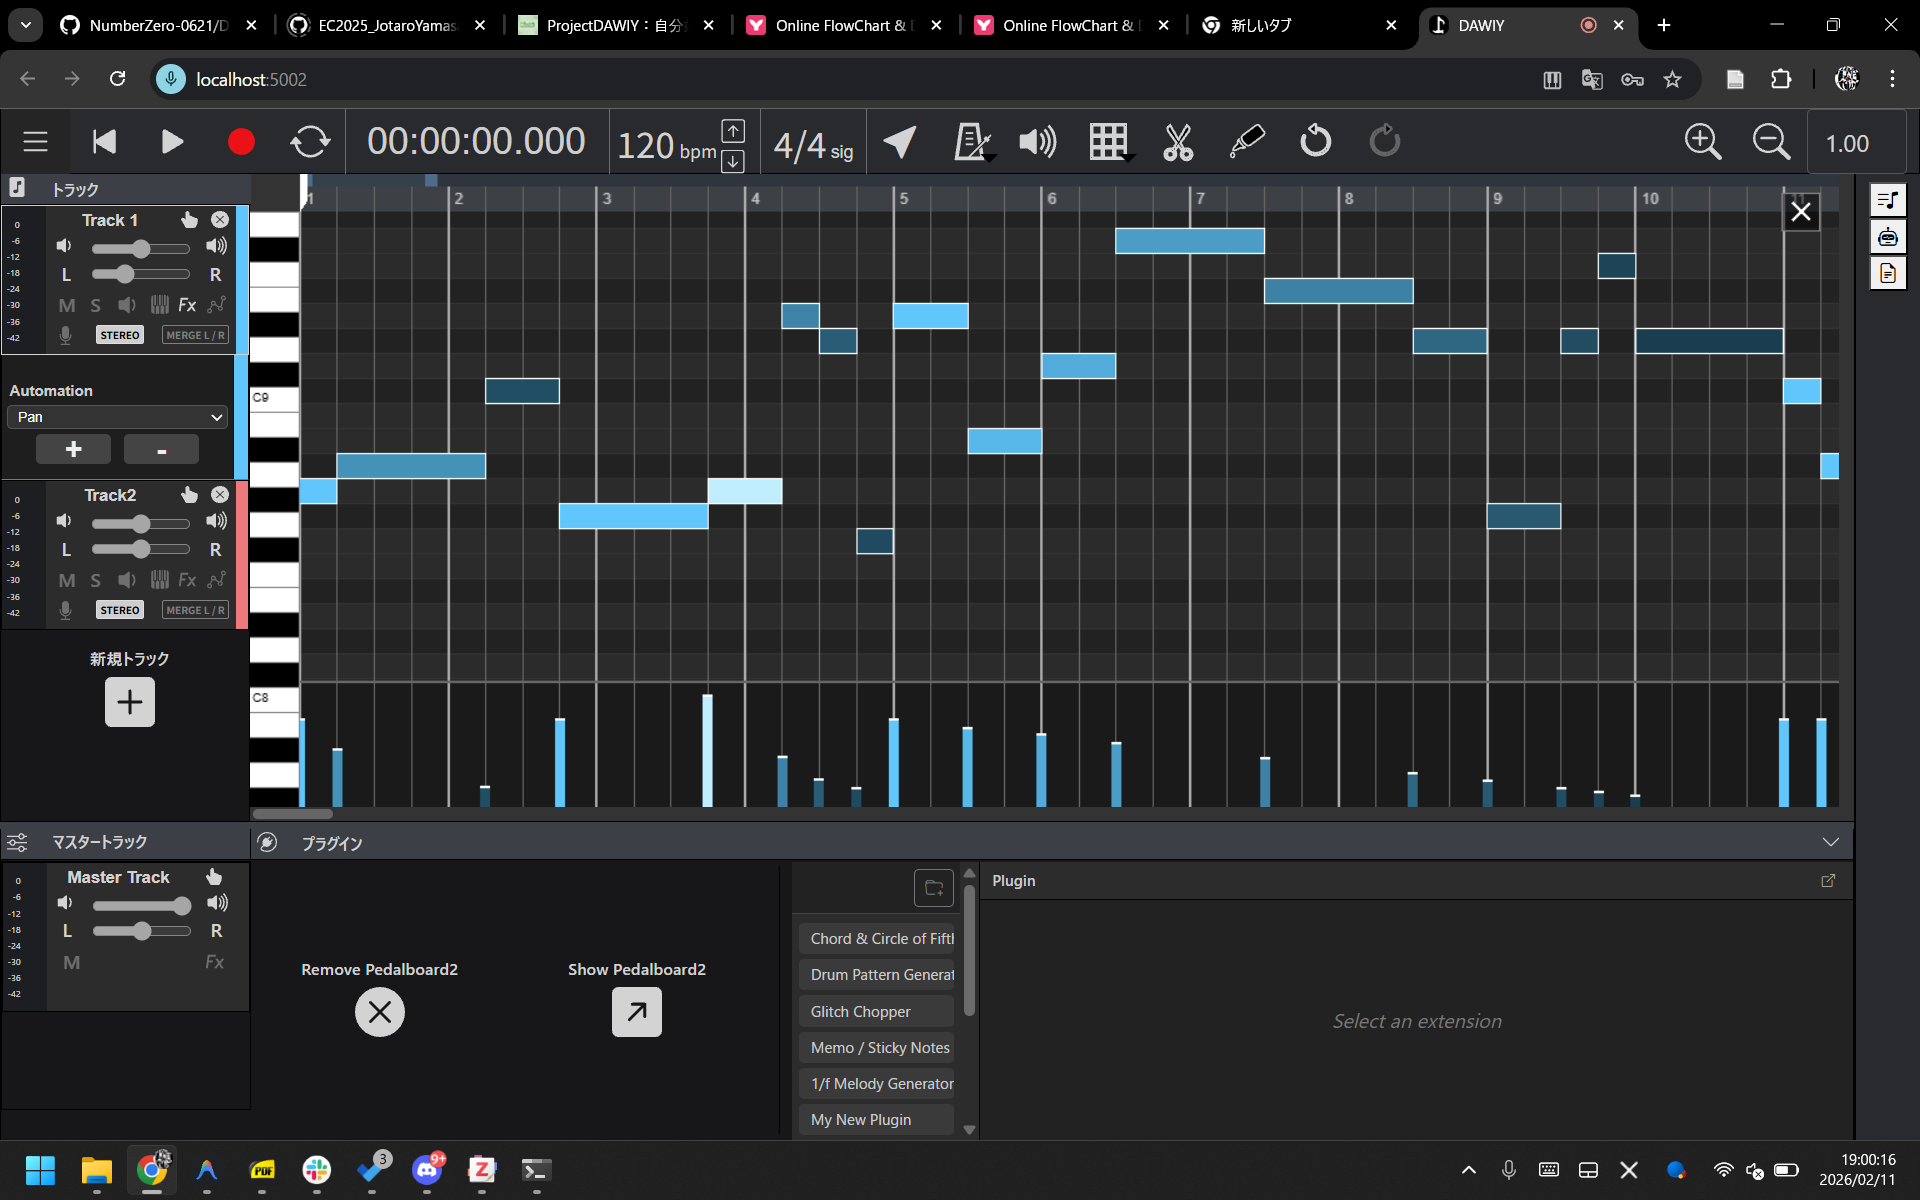
\includegraphics[width=0.9\linewidth]{../fig/pianoroll.png}
  \caption{実装したピアノロール}
  \label{fig:pianoroll}
\end{figure}

\subsection{ピアノロールの実装}
DAWとしての基本的な編集機能を提供するため，MIDIノートを視覚的に配置・編集できるピアノロール画面を実装した（\textbf{図\ref{fig:pianoroll}}）．具体的には，マウス操作によるノートの追加・削除，再生位置を示す再生バーの表示，ノートの長さの伸縮，複数ノートの範囲選択，および基本的なキーボードショートカットなどの機能を実現した．

\subsection{dawproject形式での入出力}
他のDAWとの互換性を確保するため，\texttt{dawproject}形式のプロジェクトファイルを読み込み，DAW内に展開するインポート機能を実装した．逆に，本DAW上で作成したシーケンス情報を\texttt{.dawproject}ファイルとして書き出すエクスポート機能も実装した．これにより，Studio OneやCubaseといった他の主要DAWとプロジェクトデータを交換する準備が整った．

\subsection{AIによる動的プラグイン生成機能}

\begin{figure}[tb]
  \centering
  % 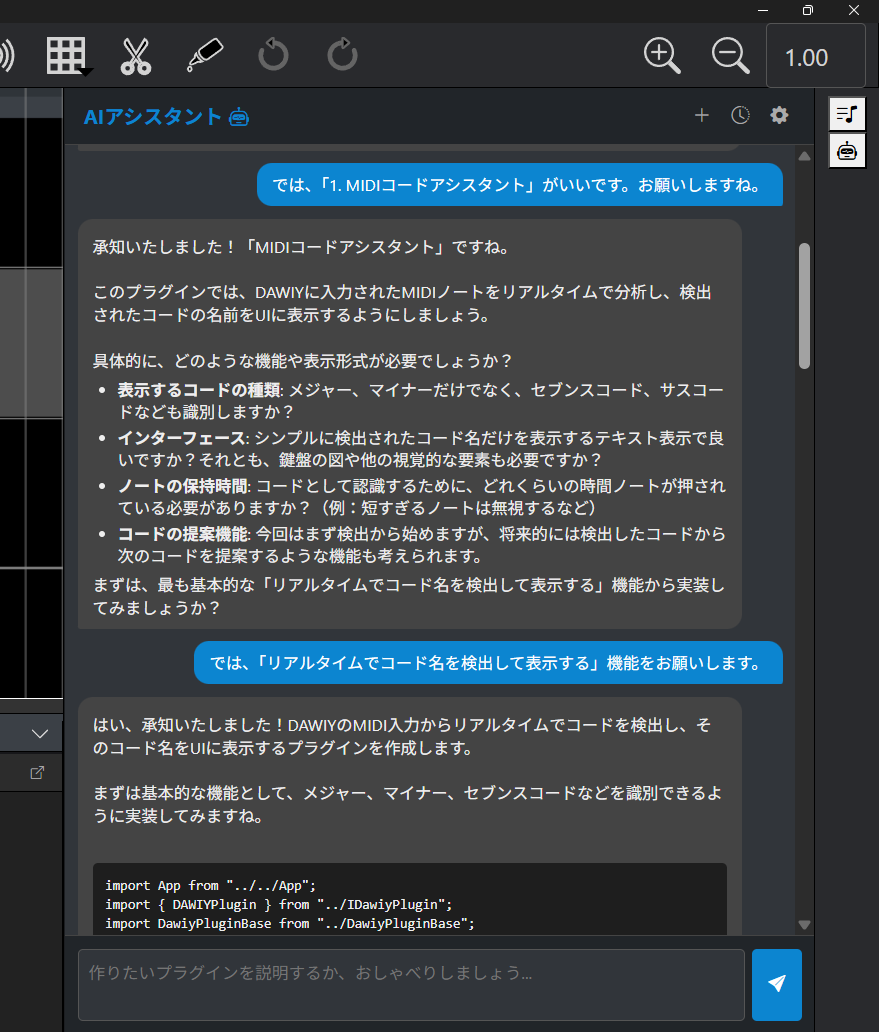
\includegraphics[width=0.9\linewidth]{../fig/ai_assistant.png} % 画像は後で差し込む
  \caption{実装したAIアシスタントのサイドバー}
  \label{fig:ai_assistant}
\end{figure}

本研究の最大の成果である，AIによるプラグイン生成機能について述べる．DAWIYの画面左側に常駐する「AIアシスタント」（サイドバー）を実装した．

\subsubsection{対話インターフェースとプロンプトエンジニアリング}
AIアシスタントは，Google Gemini APIやOpenAI API等のLLMプロバイダと連携している．ユーザが自然言語で「シンプルなボリュームコントローラーを作って」「ランダムにメロディを生成する機能が欲しい」といった要望を入力すると，システムは以下の要件を含んだシステムプロンプトと共にLLMへリクエストを送信する．

\begin{itemize}
    \item DAWIYのプラグイン基底クラス（\texttt{DawiyPluginBase}）を継承すること．
    \item 必要な装飾子（\texttt{@DAWIYPlugin}）を付与すること．
    \item 適切なライフサイクルメソッド（\texttt{onActivate}, \texttt{render}等）を実装すること．
\end{itemize}

これにより，DAWIY上で動作確実なTypeScriptコードが出力される．

\subsubsection{コードの検証と動的ロード}
生成されたコードは，クライアントサイドで簡易的なバリデーション（禁止された外部ライブラリのimportチェックなど）が行われる．問題がなければ，UI上に「Create Plugin」ボタンが表示される．
ユーザがボタンを押下すると，生成されたTypeScriptファイルと定義ファイル（plugin.json）がWebサーバへアップロードされる．DAWIYのプラグイン管理コントローラー（\texttt{DawiyPluginController}）は，これらのファイルを即座に検知・コンパイルし，ページのリロードを行うことなく動的に新しいプラグインとしてシステムに組み込む．
この一連の流れにより，ユーザはコードを一切書くことなく，対話をするだけで数秒〜数十秒で独自の機能をDAWIYに追加することが可能となった．

\section{考察}
本研究の核心であるAIによるプラグイン生成機能は，当初の「機能の自由な追加」という目標を，開発者が想定していなかったレベルで実現した．プログラミングスキルを持たないユーザでも，「欲しい機能」を言語化さえできれば，それを実際の動作機能として獲得できる点は，「DAWの民主化」における大きな進歩である．
実装した動的ロード機構により，試行錯誤のサイクル（生成→実行→修正依頼→再生成）が極めて高速に回るため，ユーザはストレスなく自分だけの制作環境を構築できる．

一方で，課題も存在する．生成されるコードの安全性（悪意あるコードや無限ループなど）の担保は現状簡易的なチェックに留まっており，サンドボックス化などのセキュリティ対策が今後の課題である．また，高度な信号処理（DSP）を伴うオーディオエフェクトの生成は，現状のLLMの能力とWeb Audio APIの複雑さの兼ね合いから，まだ精度に改善の余地がある．

\section{おわりに}
本研究では，ユーザが自由に機能をDIYできる音楽制作環境「DAWIY」の実現に向け，その基盤となるプラットフォームをWAM-Studioベースで開発した．成果として，ピアノロールによるシーケンス編集機能，\texttt{dawproject}形式によるデータ入出力機能，そしてプラグイン機構のプロトタイプを実装した．

今後の展望として，生成されたプラグインのセキュリティ向上と，より高度なDSPプラグイン生成に向けたシステムプロンプトの改良が挙げられる．また，生成されたプラグインをユーザ間で共有できるマーケットプレイス的な機能の実装も検討している．
本研究により，DAWIYは「使うDAW」から「創るDAW」へと進化し，クリエイターの創造性を拡張する新たなプラットフォームとなる可能性を示した．  % 本文は report-jotaro.tex に書く

% ==========================================
% 参考文献
% ==========================================

\bibliographystyle{ipsjunsrt}
\bibliography{../pbl2025-jotaro} % .bibファイルの名前（Zoteroからエクスポートして作る）

% ==========================================
% 付録（必要なら）
% ==========================================
% \newpage
% \appendix
% あいうえお
% \input{appendix-sample} % 付録は appendix-sample.tex に書く

\end{document}